\section{Introduction}

The notion of a balanced tensor product was first given in
\cite{etingof/fusion-cat-and-homotopy}, and mainly developed mainly in
\cite{douglas/balanced-product}. It has different interpretations in various
fields:
\begin{itemize}
  \item In the theory of topological phase, this construction corresponds to
        fusing two domains (labeled by module categories) along the domain
        wall (labeled by tensor categories) \cite{kong/topological-order}.
  \item In the theory of extended topological quantum field theory, it is the
        $1$-categorical structure of a common target $3$-category $TC$
        \cite{douglas/dualizable-tensor-categories}.
  \item In the theory of vertex operator algebra (VOA), this construction help
        study them by relating various VOAs \cite{gannon/sln-II}, and
        constructing new VOAs. % TODO Consult Terry and Harshit.
  \item In the theory of tensor category itself, it closely relates to the
        categorical center construction. In particular, the Drinfeld center
        $Z(C)$ of $C$ is equivalent to $C \boxtimes_{C \boxtimes C^{op}} C$
        \cite{kirillov/string-net-tv}
        \cite{douglas/dualizable-tensor-categories}.
\end{itemize}

Before this work, several algebraic constructions for balanced tensor products
were known, including categories of modules \cite{douglas/balanced-product},
internal Hom spaces \cite{davydov/picard}, and generalized categorical centers
\cite{etingof/fusion-cat-and-homotopy} \cite{kirillov/fact-homo-4d-tqft}
\cite{hoek/master}. These approaches well-captured the algebraic aspects of
balanced tensor products.

In this paper, we provide a topological construction based on skein theory,
which strikes a better mix between algebra and topology. This approach has at
least two advantages over previous constructions.

\subsection{Advantages}

\begin{enumerate}
  \item Its topological nature serves as the crucial element in demonstrating
        the necessity of skeins in Lurie's fully extended field theories in
        dimension $3$ \cite{lurie/tqft}.
  \item It generalizes seamlessly to balanced tensor products involving more
        than two module categories, as shown by the following expression:
        \[ {}_{A}{M}_{B} \boxtimes_{B} {}_{B}{N}_{C} \boxtimes_{{C}} {}_{C}{L}_{D} \ldots \]
\end{enumerate}

\subsection{Applications} \label{section/applications},

\begin{enumerate}
  \item \textbf{(Skein Nature of eTFTs)} In an upcoming work
        \cite{guu/tv-as-3-functor}, we build on the main result presented here
        to prove the long-anticipated theorem that the Turaev-Viro state sum
        model \cite{viro/turaev-viro-model} naturally and necessarily emerges
        from the 3-functor in the classification of fully extended field
        theories \cite{lurie/tqft}.
  \item \textbf{(No-Go: Detection of Exotic Smooth Structures)} We anticipate
        that this approach can be extended to its 4D analogue, the
        Crane-Yetter model. Additionally, this strategy should apply to a
        broader generalization based on fusion 2-categories, as explored in
        \cite{douglas/fusion-2-cat-4d-tqft}. Proving this would lend support
        to the conjecture proposed there, which suggests that despite the
        construction's generality and power, it remains an extended
        topological field theory and therefore cannot detect exotic structures
        \cite{reutter/no-go-exotic}.
  \item \textbf{(Factorization Homology)} The main result of this paper
        provides a simple reproof of the result in
        \cite{kirillov/fact-homo-4d-tqft} that shows equivalence between the
        Crane-Yetter model and factorization homology
        \cite{ayala/factorization-homology} in $4$D (the excision property).
  \item \textbf{(Defected TFTs)} We expect work being useful in the study of
        defect field theories, such as in \cite{meusburger/defect-tv}.
  \item \textbf{(Computations in Tensor / Higher Categories)} Given that the
        Drinfeld center is a specific instance of the balanced tensor product,
        we expect this paper will contribute to recent advancements,
        particularly the explicit computation of centers as explored in
        \cite{maurer/computing-center}, and further develop the computational
        aspects of balanced tensor products.
\end{enumerate}

\subsection{Conventions}\label{subsection/conventions}

For simplicity, throughout the whole paper, unless otherwise mentioned, we assume the following.
\begin{enumerate}
  \item The base field is the complex number field $\mathbb{C}$.
  \item Every tensor category is finite, semisimple, pivotal, and defined over $\mathbb{C}$.
  \item Every (bi-)module category is finite, semisimple, and defined over
  $\mathbb{C}$.
  \item Every (bi-)module category functor is right exact (following
        \cite{douglas/balanced-product}).
        % TODO Why do we need right-exactness? Does this mean we have to check
        % right-exactness for our result as well?
\end{enumerate}

\subsection{A Note to Experts}\label{subsection/a-note-to-experts}

The main theorem provides an algebraic model for balanced tensor products with
mathematical rigor, utilizing the skein construction. We do not claim to
introduce novel ideas here: This approach closely mirrors the domain-wall
perspective in topological phase theory, as outlined in
\cite{kong/topological-order}. In fact, the essential techniques have been
used in many places to study the Drinfeld center
$Z(C) \simeq C \boxtimes_{CC} C$ (e.g. \cite{kirillov/string-net-tv}). This
work is merely a generalization of it to the context of field theories with
defects.

In this work, we assume ideal conditions—finiteness, semisimplicity, and
pivotality (see \ref{subsection/conventions}). While it is both possible and
beneficial to relax some of these assumptions, for simplicity, we leave such
generalizations for future work. For example, we expect our proof works even
if pivotality is demoted to rigidity.

\section{Balanced Tensor Product (Algebra)}\label{section/balanced-tensor-product}

\noindent In this section we recall the definition of balanced tensor product
from \cite{douglas/balanced-product}.

\begin{definition} (Balanced Module Category Functor)

  \noindent Let $C, D, E$ be tensor categories. Let $_{C}M_{D}$ be a
  $C{\text -}D$ bimodule category, $_{D}N_{E}$ be a $D{\text -}E$ bimodule
  category, $_{C}L_{E}$ be a $C{\text -}E$ bimodule category. \quad Then a
  $D$-balanced $C{\text -}E$ bimodule category functor (from $M \times N$ to $L$)
  is a pair
  \[(M \times N \xrightarrow{F} L, \alpha)\] where $F$ is a bilinear $C{\text -}E$
  bimodule category functor and $\alpha$ is a natural isomorphism between the
  following two functors from $M \times D \times N$ to $L$
  \[
    \begin{tikzcd}
      M \times D \times N \arrow[r] \arrow[dr] &
      M \times N \arrow[d, Rightarrow, "\alpha"] \arrow[r, "F"] &
      L \\
      & M \times N \arrow[ur, "F"'] \\
    \end{tikzcd}
  \]
  where the object $(m,d,n)$ in $M \times D \times N$ is sent by the first
  upper arrow to $(m \lhd d, n)$, and by the first lower arrow to $(m, d \rhd n)$.
\end{definition}

% TODO
% \begin{remark}
%   The triangle and pentagonal identities for $D$ is automatically satisfied
%   [TODO: see Jin's note 20240906-110000 p.2].
% \end{remark}

\begin{definition} (Balanced Natural Transformation)

  \noindent Let $C, D, E$ be tensor categories. Let $_{C}M_{D}$ be a $C{\text -}D$
  bimodule category, $_{D}N_{E}$ be a $D{\text -}E$ bimodule category, $_{C}L_{E}$ be
  a $C{\text -}E$ bimodule category. Let $F, F'$ be $D$-balanced $C{\text -}E$ bimodule
  category functors from $M \times N$ to $L$. A $D$-balanced transformation
  from $F$ to $F'$ is a natural transformation $ F \xrightarrow{\eta} F'$ such
  that the following diagram commutes (in a naturally compatible way with the
  $C{\text -}E$ bimodule structures.)

  \[
    \begin{tikzcd}
      F(m \lhd c, n) \arrow[r, "\alpha_{m,c,n}"] \arrow[d, "\eta_{m \lhd c, n}"'] &
      F(m, c \rhd n) \arrow[d, "\eta_{m, c \rhd n}"] \\
      F'(m \lhd c, n) \arrow[r, "\alpha_{m,c,n}'"'] &
      F'(m, c \rhd n)
    \end{tikzcd}
  \]
\end{definition}

\begin{definition} (Category of Balanced Functors)

  \noindent Let $C, D, E$ be tensor categories. Let $_{C}M_{D}$ be a
  $C{\text -}D$ bimodule category, $_{D}N_{E}$ be a $D{\text -}E$ bimodule
  category, $_{C}L_{E}$ be a $C{\text -}E$ bimodule category. Let $F, F'$ be
  $D$-balanced $C{\text -}E$ bimodule category functors from $M \times N$ to $L$.
  \quad Then the category of balanced functors
  $Fun^{D{\text -}bal}_{C,E}(M \times N, L)$ is defined to be the category whose
  objects are $D$-balanced $C{\text -}E$ bimodule category functors
  $M \times N \to L$ and whose morphisms are $D$-balanced natural transformations.
\end{definition}

% TODO: In this definition, I need M, N are semisimple already. But add
% a later remark saying that this can be circumvented.

\begin{definition} (Balanced Tensor Product)

  \noindent Let $C, D, E$ be tensor categories. Let $_{C}M_{D}$ be a
  $C{\text -}D$ bimodule category, and $_{D}N_{E}$ be a $D{\text -}E$ bimodule
  category. \quad Then the balanced tensor product $_{C}(M \boxtimes_{D} N)_{E}$ is
  the $C{\text -}E$ bimodule category defined as the initial $D$-balanced
  module functor from $M \times N$; i.e. for each map from $M \times N$ to some
  $C{\text -}E$ bimodule category $L$, there exists a unique $C{\text -}E$
  bimodule category functor $G$ such that the following diagram commutes,

  \[
    \begin{tikzcd}
      M \times N \arrow[r, "F"] \arrow[d, "\boxtimes_{D}"'] & L \\
      _{C}(M \boxtimes_{D} N)_{E} \arrow[ur, "G"']
    \end{tikzcd}
  \]

  \noindent and that it induces an equivalence of categories
  \[Fun_{C,E}(M \boxtimes_{D} N, L) \simeq Fun_{C,E}^{D{\text -}bal}(M \times N, L).\]
\end{definition}

\section{Skein Construction (Topology)}\label{section/skein-construction}

\begin{definition} (Pre-Skein Category)

  \noindent Let $C$ be a tensor category. Let $M_{C}$ and $ _{C}N$ be module
  categories. \quad Define the pre-skein category $p.sk(M,C,N)$ to be the
  category $P$ with $Obj(P) = Obj(M \boxtimes N)$, and the morphism spaces
  $Mor_{P}((m \boxtimes n), (m' \boxtimes n'))$ are defined to be the vector space
  $(V \,/ \sim)$, where
  \[
    V := \oplus_{c,\overline{c} \in Obj(C)} Hom_{M}(m, m' \lhd c) \otimes Hom_{C}(c,\overline{c}) \otimes Hom_{N} (\overline{c} \rhd n, n'),
  \]
  and the relations $\sim$ are generated by the following types of relations
  \begin{align}
    \phi \otimes (\overline{\pi} \circ \pi) \otimes \psi &- (\phi_{\pi} \otimes \overline{\pi} \otimes \psi) \label{relation/a} \\
    \phi \otimes (\overline{\pi} \circ \pi) \otimes \psi &- (\phi \otimes \pi \otimes {}_{\overline{\pi}}\psi) \label{relation/b},
  \end{align}
  where
  \begin{align}
    \phi_{\pi}  &:= \left( m \xrightarrow{\phi} m' \lhd c \xrightarrow{1_{m'} \lhd \pi} m' \lhd c' \right)\\
    {}_{\overline{\pi}}\psi &:= \left( \overline{c} \rhd n \xrightarrow{\overline{\pi} \rhd 1_{n}} \overline{\overline{c}} \rhd n \xrightarrow{\psi} n' \right)
  \end{align}

  % TODO: Make a better picture.
  \begin{center}
    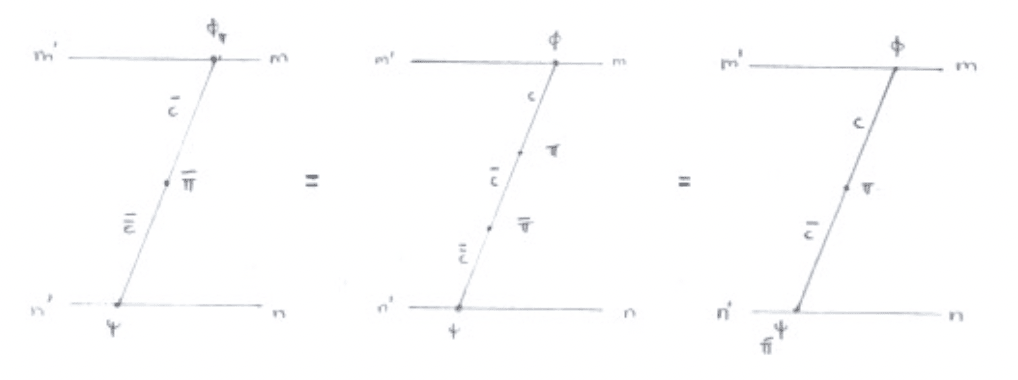
\includegraphics[width=18cm]{1}
  \end{center}

  \noindent We define the composition on the level of $V$. It is
  straightforward to check that it descends properly to $(V \, / \sim)$ using
  the $2$-categorically compositional nature of tensor categories.
  % TODO: If have time, add a complete proof for this claim, perhaps in the appendix.
  The composition
  \[
    (\phi' \otimes \pi' \otimes \psi' ) \circ (\phi \otimes \pi \otimes \psi)
  \]
  is defined to be $(\phi'' \otimes \pi'' \otimes \psi'')$ where
  \begin{itemize}
    \item
    $\pi'' \in Hom_{C}(c' \otimes c, \overline{c}' \otimes \overline{c})$ is equal to
    \[
      c' \otimes c \xrightarrow{\pi' \otimes \pi} \overline{c'} \otimes \overline{c},
    \]
    \item
    \noindent $\phi'' \in Hom_{M}(m, m'' \lhd (c' \otimes c))$ is equal to
    \[
      m \xrightarrow{\phi} m' \lhd c \xrightarrow{\phi' \lhd 1_{c}} (m'' \lhd c') \lhd c \xrightarrow[\sim]{\alpha} m'' \lhd (c' \otimes c),
    \]
    \item
    \noindent $\psi'' \in Hom_{N}((\overline{c}' \otimes \overline{c}) \rhd n, n'')$ is equal to
    \[
      (\overline{c}' \otimes \overline{c}) \rhd n \xrightarrow[\sim]{\alpha} \overline{c}' \rhd (\overline{c} \rhd n) \xrightarrow{1_{\overline{c}'} \rhd \psi} \overline{c}' \rhd n' \xrightarrow{\psi'} n''.
    \]
  \end{itemize}

  % TODO: Make a better picture.
  \begin{center}
    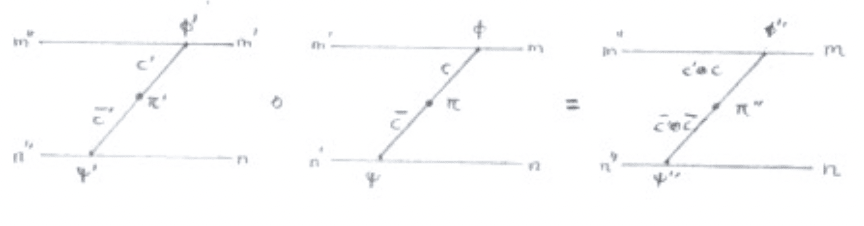
\includegraphics[width=18cm]{2}
  \end{center}

  \noindent Finally, extend the definition of the morphism spaces to those between
  general objects via direct sum.

\end{definition}

\begin{notation} (${}^{m'}_{n'}I^{m}_{n}$)

  \noindent Denote the equivalence class of the vector
  $(\phi \otimes \pi \otimes \psi) \in V$ by
  \[\III{m'}{n'}{m}{n}{\phi}{\psi}{c}{\pi}{c'}.\]
  When $m' = m$ and $n' = n$, we omit the primed symbols and write
  \[
    \III{}{}{m}{n}{\phi}{\psi}{c}{\pi}{c'} :=
    \III{m}{n}{m}{n}{\phi}{\psi}{c}{\pi}{c'}.
  \]
  When $\pi = 1_{c}$ (thus $c' = c$), we abbreviate it further to
  \[
    \II{m'}{n'}{m}{n}{\phi}{\psi}{c} :=
    \III{m'}{n'}{m}{n}{\phi}{\psi}{c}{1_{c}}{c},
  \]
  and
  \[
    \II{}{}{m}{n}{\phi}{\psi}{c} :=
    \III{m}{n}{m}{n}{\phi}{\psi}{c}{1_{c}}{c}.
  \]
\end{notation}

\begin{remark}\label{remark/skein-nature-of-the-notation-I} (Skein Nature of the Notation ${}^{m'}_{n'}I^{m}_{n}$)

  \noindent Informally yet instructively, it is helpful to view
  $\III{m'}{n'}{m}{n}{\phi}{\psi}{c}{\pi}{c'}$ as a skein flowing from the right to
  the left, starting from $m \boxtimes n$ to $m' \boxtimes n'$, passing through $\phi \boxtimes \psi$;
  during the process, the upper strain emits a particle $c$ at $\phi$, which
  transforms to via $\pi$ to $\overline{c}$, and hits the lower strain at
  $\psi$. Hence under the defined composition rule (see the equation for
  $\phi'' \otimes \pi'' \otimes \psi''$ above), we have
  \[
    \III{m''}{n''}{m'}{n'}{\phi'}{\psi'}{c'}{\pi'}{\overline{c}'} \circ
    \III{m'}{n'}{m}{n}{\phi}{\psi}{c}{\pi}{\overline{c}} =
    \III{m''}{n''}{m}{n}{\phi''}{\psi'}{c' \otimes c}{\pi''}{\overline{c}' \otimes \overline{c}}.
  \]
\end{remark}

\begin{remark}\label{remark/hom-space-reduction} (Hom Space Reduction)

  \noindent By the relations in the definition, the transformation
  \[
    \pi = 1_{\overline{c}} \circ \pi = \pi \circ 1_{c}
  \]
  can be absorbed into each of the strain, so
  \[
    \II{m'}{n'}{m}{n}{\phi}{{}_{\pi}\psi}{c} =
    \III{m'}{n'}{m}{n}{\phi}{{}_{\pi}\psi}{c}{1_{c}}{c} =
    \III{m'}{n'}{m}{n}{\phi}{\psi}{c}{\pi}{c'} =
    \III{m'}{n'}{m}{n}{\phi_{\pi}}{\psi}{c'}{1_{c'}}{c'} =
    \II{m'}{n'}{m}{n}{\phi_{\pi}}{\psi}{c'}.
  \]

  \noindent Furthermore, if $c \simeq \oplus_{i=1}^{l} c_{i}$, then
  \[
    \II{m'}{n'}{m}{n}{\phi}{\psi}{c} = \II{m'}{n'}{m}{n}{\phi}{\psi}{\oplus_{i=1}^{l} c_{i}} = \sum_{j=1}^{l} \III{m'}{n'}{m}{n}{\phi_{j}}{\psi}{c_{j}}{\iota_{j}}{\oplus_{i=1}^{l} c_{i}} =
    \sum_{j=1}^{l}\II{m'}{n'}{m}{n}{\phi_{j}}{\psi_{j}}{c_{j}},
  \]
  where $\iota_{j}$ denotes the $j$-th embedding map from $c_{j}$ to
  $\oplus_{i=1}^{l}c_{i}$, and the $\phi_{j}, \psi_{j}$'s denote the $j$-th
  projection of $\phi, \psi$ respectively. In particular, when
  $c \simeq x^{\oplus l}$, the this gives a reduction from
  \[
    Hom_{M}(m, m' \rhd x^{\oplus l}) \otimes Hom_{C}(x^{\oplus l}, x^{\oplus l}) \otimes Hom_{N} (x^{\oplus l} \lhd n, n')
  \]
  to
  \[
    Hom_{M}(m, m' \rhd x) \otimes Hom_{C}(x, x) \otimes Hom_{N} (x \lhd n, n').
  \]
  It is helpful to regard the result as the ``inner product'' of $\phi$ and $\psi$.
\end{remark}

\noindent The hom vector spaces are finite dimensional. An explicit basis is
constructed in \ref{proposition/basis-theorem}.

\begin{definition} \label{definition/karoubi-completion} (Karoubi Completion)

  \noindent Let $C$ be a category. \quad The Karoubi completion $Kar(C)$ of
  $C$ is defined to be the category with
  \[
    Obj(Kar(C)) = \{(c, f) \,|\, c \in Obj(C), f \in End_{C}(c), f = f^{2}\}
  \] and
  \[
    Mor_{Kar(C)}((c,f), (c', f')) = \{\overline{f} \in Hom_{C}(c,c') \,|\, \overline{f}f = \overline{f} = f'\overline{f}\},
  \]
  with the obvious composition rule.
\end{definition}

\begin{remark} \label{remark/karoubi-retract} (Karoubi Retracts)

  \noindent It is straightforward to check that every object $(c,f)$ in
  $Kar(C)$ is a retract of the original object $c = (c, 1_{c})$. So we have
  \[
    (c, f) \xrightarrow{\iota} c = (c, 1_{c}) \xrightarrow{\pi} (c, f).
  \]
\end{remark}

\begin{definition}\label{definition/skein-category} (Skein Category)

  \noindent Let $C$ be a tensor category. Let $M_{C}$ and $_{C}N$ be module
  categories. \quad Define the skein category $sk(M,C,N)$ to the Karoubi
  completion of its pre-skein category
  \[
    sk(M,C,N) := Kar(p.sk(M,C,N)).
  \]
  \noindent Thus, a typical object of the skein category $sk(M,C,N)$ is the
  direct sum of some idempotent skeins $\II{m}{n}{m}{n}{\phi}{\psi}{c}$
  ($m \in Obj(M), n \in Obj(N)$). The skein category is obviously a linear
  category.

  More generally, for any $n \in \mathbb{N}$, let
  $C_{0}, C_{1}, \ldots, C_{n}$ be tensor categories. Let
  ${}_{C_{0}}M^{1}_{C_{1}}, \, {}_{C_{1}}M^{2}_{C_{2}}, \ldots, {}_{C_{n{\text -}1}}M^{n}_{C_{n}}$
  be bimodule categories. One can in a similar way define the
  $C_{0}{\text -}C_{n}$ bimodule category
  \[
    sk(M^{1}, C_{1}, M^{2}, C_{2}, M^{3}, \ldots, C_{n{\text -}1}, M^{n}).
  \]
  % TODO: Make a better picture.
  \begin{center}
    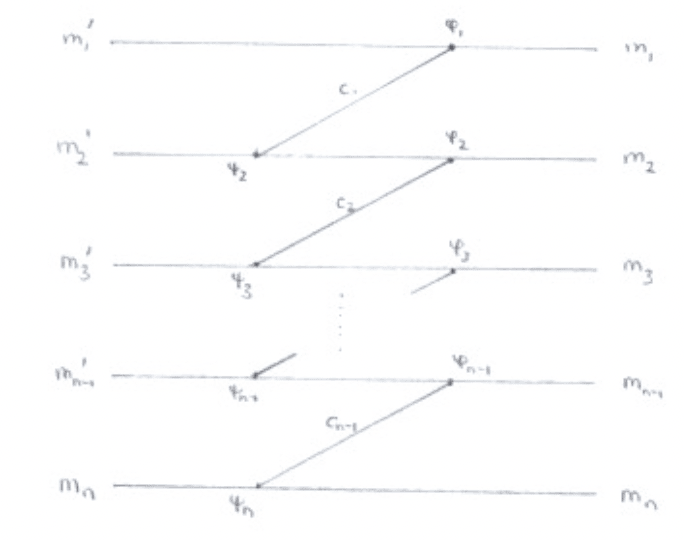
\includegraphics[width=12cm]{3}
  \end{center}

\end{definition}

\begin{definition} \label{definition/induced-functor-on-skein-category} (Induced Functor on Skein Category)

  \noindent Assume the notation in \ref{definition/skein-category}. Let
  $1 \leq i \leq n$, and let $F: M^{i} \to M'^{i}$ be a
  $C_{i{\text -}1}{\text -}C_{i}$ bimodule category functor. \quad Then $F$
  naturally induces a linear functor between the skein categories
  \[
    sk(M^{1}, C_{1}, M^{2}, C_{2}, M^{3}, \ldots M^{i} \ldots, C_{n{\text -}1}, M^{n})
    \xrightarrow{F}
    sk(M^{1}, C_{1}, M^{2}, C_{2}, M^{3}, \ldots M'^{i} \ldots, C_{n{\text -}1}, M^{n}).
  \]
  For example, if $n=2$, $M^{1} = M$, $M^{2} = N$, $C^{1} = C$, $N \xrightarrow{F} N'$
  (with the left $C$-module structure given by $\alpha$), then we have an
  induced linear functor $sk(M,C,N) \to sk(M,C,N')$ sending the objects and morphisms via the map:
  \[
    \II{m'}{n'}{m}{n}{\phi}{\psi}{c}
    \quad \mapsto \quad
    \II{m'}{F(n')}{m}{F(n)}{\phi}{F(\psi) \circ \alpha}{c}.
  \]
\end{definition}

\noindent The main result of this paper is to show that the skein category
$sk(M,C,N)$ is equivalent to $M \boxtimes_{C} N$, and that the induced functor $M \boxtimes_{C} N \to M \boxtimes_{C} N'$
coincides with the one in \ref{definition/induced-functor-on-skein-category}
(proven in \ref{lemma/main-lemma}, \ref{theorem/main-theorem}). A necessary
ingredient is the canonical map $\boxtimes_{C}$ given in the defining universal
property.

\begin{definition}\label{definition/canonical-map} (Canonical Map $\boxtimes_{C}$)

  \noindent Let $C$ be a tensor category, and $M_{C}, _{C}N$ be module
  categories. \quad Define the functor
  \[
    M \times N \xrightarrow{\boxtimes_{C}} sk(M,C,N)
  \]
  to send the object $(m,n)$ to the object $\II{m}{n}{m}{n}{1_{m}}{1_{n}}{1_{1}}$, and the morphism
  \[
    (m,n) \xrightarrow{(\phi, \psi)} (m', n')
  \]
  to the morphism $\II{m'}{n'}{m}{n}{\phi}{\psi}{1_{1}}$.
\end{definition}

\noindent From the main theorem, we must have $sk(M,C,C) \simeq M$. To quickly
convince the reader that the main theorem is true before it is proven, we
provide another direct proof for this equivalence in the appendix (cf
\ref{proposition/degenerated-main-theorem}).

\hfill\break
\noindent We prove another lemma that will be useful later.

\begin{lemma}\label{lemma/I-provides-subobject} (Objects are Retracts)

  \noindent Let $C$ be a tensor category, and $M_{C}, _{C}N$ be module
  categories. \quad Then any typical object $\II{}{}{m}{n}{\phi}{\psi}{c}$ in
  $sk(M,C,N)$ is a retract (in particular, a subobject) of the canonical
  object $\boxtimes_{C}((m,n)) = \II{}{}{m}{n}{1_{m}}{1_{n}}{1}$.
\end{lemma}
\begin{proof}
  This directly follows from \ref{remark/karoubi-retract}.
\end{proof}

\section{Proof of the Main Equivalence Theorem}\label{section/proof-of-equivalence}

Unless specified otherwise, throughout this section, let $C, D, E$ be tensor
categories, let $M_{C}$ and $_{C}N$ be module categories, and let $L$ be a
linear category. We prove our main theorem (\ref{theorem/main-theorem}) in this section, justifying
that the skein construction $sk(M,C,N)$ is isomorphic to $M \boxtimes_{C} N$, and the
obvious generalization to the case of more bimodule categories.

\begin{lemma}\label{lemma/construction-of-theta} (Construction of $\Theta$)

  \noindent There exists a linear functor
  \[
    \Theta: Fun(sk(M,C,N), L) \to Fun^{C{\text -}bal}(M \times N, L).
  \]
\end{lemma}

\noindent We construct $\Theta$ explicitly in the proof.

\begin{proof}
  \noindent (Object) Let $G$ be an object of the domain. Define $\Theta(G)$ to
  be $F := G \circ \boxtimes_{C} \in Fun(M \times N, L)$. We shall provide the
  balanced structure $\alpha$ for $F$, so that $(F, \alpha)$ is $C$-balanced. 
  We need to provide the $C$-balanced data for $F$:
  \[
    \alpha_{m,c,n}: F(m \lhd c, n) =
    G(\II{}{}{mc}{n}{1}{1}{1})
    \xrightarrow{\sim} G(\II{}{}{m}{cn}{1}{1}{1})
    = F(m, c \rhd n),
  \]
  which is clearly satisfied by $G(\II{m}{cn}{mc}{n}{1}{1}{c}).$ So defined
  $\alpha$ is clearly natural.

  \noindent (Morphism) Let $G \xrightarrow{\eta} G'$ be a morphism in
  $Fun(sk(M,C,N), L)$. Its image under $\Theta$ is simply the horizontal
  composition $\eta \star (1_{\boxtimes_{C}})$. The remaining commutativity to be checked
  % TODO: cf p11 of Jin's note 20240906-110000
  is a direct consequence of $\eta$'s naturality.
\end{proof}

\begin{lemma}\label{lemma/theta-is-faithful} ($\Theta$ is faithful)

  \noindent The linear functor $\Theta$ (cf. \ref{lemma/construction-of-theta}) is faithful.
\end{lemma}

\begin{proof}
  (We use the same notation found in this section.) This amounts to showing
  that the following map is an injective linear map:
  \[
    (G \xrightarrow{\eta} G') \mapsto (F \xrightarrow{\Theta(\eta) = \eta \star (1_{\boxtimes_{C}})} F').
  \]
  It is clearly linear. For injectivity, we notice that whenever we have
  linear functors
  \[
    X \xrightarrow{f} Y,\quad Y \xrightarrow{g, g'} Z,
  \]
  and a linear natural transformation $\eta: g \to g'$, then the map $(\eta \mapsto \eta \star 1_{f})$ is injective is equivalent to
  \[
    (\forall x \in Obj(X), \eta_{f(x)} = 0) \Rightarrow (\forall y \in Obj(Y), \eta_{y} = 0).
  \]
  This holds if $f$ is surjective on objects. However, in our case
  $f = \boxtimes_{C}$ is not as strong. Fortunately, clearly it also holds if
  $f$ is almost-surjective, in the sense that each $y \in Obj(Y)$ has an
  $x \in Obj(X)$ such that $y$ is a subobject of $f(X)$. Indeed,
  \[
    1_{g(y)} = g(1_{y}) = g(\pi_{y} \circ \iota_{y}),
  \]
  so
  \[
    (g(y) \xrightarrow{\eta_{y}} g'(y)) = \eta_{y} \circ 1_{g(y)} = \eta_{y} \circ g(\pi \circ \iota) = g(\pi) \circ \eta_{f(x)} \circ g(\iota) = g(\pi) \circ 0 \circ g(\iota) = 0.
  \]
  This applies to our case by putting $f = \boxtimes_{C}$ and $g = G$, because
  each object $\II{}{}{m}{n}{\phi}{\psi}{c}$ is clearly a subobject of
  $\boxtimes_{C}(m,n) = \II{}{}{m}{n}{1}{1}{1}$. Therefore, $\Theta$ is faithful.
\end{proof}

\begin{lemma}\label{lemma/theta-is-full} ($\Theta$ is full)

  \noindent The linear functor $\Theta$ (cf. \ref{lemma/construction-of-theta}) is full.
\end{lemma}

\begin{proof}
  We need to show that for any $C$-balanced natural transformation
  \[
    \nu: G \circ \boxtimes_{C} = \Theta(G) \to \Theta(G') = G' \circ \boxtimes_{C}
  \]
  there is $\mu: G \to G'$ such that $\nu = \mu \star 1_{\boxtimes_{C}}$. The data $\nu$ are the maps
  \[
    \nu_{(m,n)}: G(\II{}{}{m}{n}{1}{1}{1}) \to G'(\II{}{}{m}{n}{1}{1}{1}).
  \]
  We only need to extend these data to all objects in $sk(M,C,N)$, i.e. define compatible maps
  \[
    \nu_{\II{}{}{m}{n}{\phi}{\psi}{c}}: G(\II{}{}{m}{n}{\phi}{\psi}{c}) \to G'(\II{}{}{m}{n}{\phi}{\psi}{c}).
  \]
  It is straightforward to check that the following works:
  \[
    \nu_{\II{}{}{m}{n}{\phi}{\psi}{c}}:= G(\II{}{}{m}{n}{\phi}{\psi}{c})
    \xrightarrow{G(\iota)}
    G(\II{}{}{m}{n}{1}{1}{1})
    \xrightarrow{\nu_{(m,n)}}
    G'(\II{}{}{m}{n}{1}{1}{1})
    \xrightarrow{G'(\pi)}
    G'(\II{}{}{m}{n}{\phi}{\psi}{c}),
  \]
  where $\iota$ and $\pi$ are the inclusion and projection (see
  Lemma \ref{lemma/I-provides-subobject}).
\end{proof}

\noindent To prove that $\Theta$ is essentially surjective, we need the following
lemma.

\begin{lemma} (Images of skeins) \label{lemma/image-of-skein}
  % TODO: Discussion: Can we relax conditions? We need to use the basis theorem,
  % so it seems that we must require semisimplicity here.

  \noindent
  Let $(F,\alpha) \in Fun^{C{\text -}bal}(M \times N, L)$. For each morphism
  in $sk(M,C,N)$ of the form $\III{m'}{n'}{m}{n}{\phi}{\psi}{c}{\pi}{c'}$,
  define the image of it under $\tilde{F}$ to be the composed morphism
  \[
    F(m,n)
    \xrightarrow{F(\phi \times 1)}
    F(m' \lhd c, n)
    \xrightarrow{F((1 \lhd \pi) \times 1)}
    F(m' \lhd c', n)
    \xrightarrow[\sim]{\alpha}
    F(m', c' \rhd n)
    \xrightarrow{F(1 \times \psi)}
    F(m',n').
  \]
  Suppose we have two skeins $\II{m'}{n'}{m}{n}{\phi}{\psi}{c}$ and
  $ \II{m'}{n'}{m}{n}{\phi'}{\psi'}{c'}$ as identical morphisms in $sk(M,C,N)$
  (recall the definitional relations (\ref{relation/a}) (\ref{relation/b})).

  \noindent Then
  \begin{equation} \label{eqn/a}
    \tilde{F}(\II{m'}{n'}{m}{n}{\phi}{\psi}{c}) = \tilde{F}(\II{m'}{n'}{m}{n}{\phi'}{\psi'}{c'}).
  \end{equation}
  Moreover, $\tilde{F}$ preserves compositions, i.e.
  \begin{equation} \label{eqn/b}
    \tilde{F}(\II{m''}{n''}{m'}{n'}{\overline{\phi}}{\overline{\psi}}{\overline{c}} \circ \II{m'}{n'}{m}{n}{\phi}{\psi}{c})
    = \tilde{F}(\II{m''}{n''}{m'}{n'}{\overline{\phi}}{\overline{\psi}}{\overline{c}})
    \circ
    \tilde{F}(\II{m'}{n'}{m}{n}{\phi}{\psi}{c}).
  \end{equation}
\end{lemma}

\begin{proof}
  To prove the first statement (\ref{eqn/a}), check the equality against the
  definitional relations (\ref{relation/a}) (\ref{relation/b}).

  \noindent To prove the second statement (\ref{eqn/b}), note that the
  left-hand-side is
  $\tilde{F}(\II{m''}{n'}{m}{n}{\overline{\phi} \otimes \phi}{\overline{\psi} \otimes \psi}{\overline{c} \otimes c}),$
  which is
  \begin{multline*}
    F(m,n)
    \xrightarrow{F(\phi \times 1)}
    F(m' \lhd c, n)
    \xrightarrow{F((\overline{\phi} \lhd 1) \times 1)} \\
    F((m'' \lhd \overline{c}) \lhd c, n)
    \xrightarrow[\sim]{}
    F((m'' \lhd (\overline{c} \otimes c)), n)
    \xrightarrow[\sim]{\alpha}
    F(m'', (\overline{c} \otimes c) \rhd n)
    \xrightarrow[\sim]{}
    F(m'', \overline{c} \rhd (c \rhd n)) \\
    \xrightarrow{F(1 \times (1 \rhd \psi))}
    F(m'', \overline{c} \rhd n')
    \xrightarrow{F(1 \times \overline{\psi})}
    F(m'',n'').
  \end{multline*}
  On the other hand, the right-hand-side is
  \begin{multline*}
    F(m,n)
    \xrightarrow{F(\phi \times 1)}
    F(m' \lhd c, n)
    \xrightarrow[\sim]{\alpha} \\
    F(m', c \rhd n)
    \xrightarrow{F(1 \times \psi)}
    F(m', n')
    \xrightarrow{F(\overline{\phi} \times 1)}
    F(m'' \rhd \overline{c}, n') \\
    \xrightarrow[\sim]{\alpha}
    F(m'', \overline{c} \lhd n')
    \xrightarrow{F(1 \times \overline{\psi})}
    F(m'',n'').
  \end{multline*}
  To prove that they are equal, we can omit their first and their last arrows. Note that the composed arrow in left-hand-side $F(m' \lhd c, n) \to F(m', \overline{c} \rhd (c \rhd n))$ is, by the naturality of $\alpha$, equal to
  \[
    F(m' \lhd c, n)
    \xrightarrow[\sim]{\alpha}
    F(m', c \rhd n)
    \xrightarrow{F(\overline{\phi} \times 1)}
    F(m'' \lhd \overline{c}, c \rhd n)
    \xrightarrow[\sim]{\alpha}
    F(m'', \overline{c} \rhd (c \rhd n)).
  \]
  Compose this with
  \[
    F(m'', \overline{c} \rhd (c \rhd n))
    \xrightarrow{F(1 \times (1 \rhd \psi))}
    F(m', \overline{c} \rhd n'),
  \]
  then we get
  \[
    F(m' \lhd c, n)
    \xrightarrow[\sim]{\alpha}
    F(m', c \rhd n)
    \xrightarrow{F(\overline{\phi} \times 1)}
    F(m'' \lhd \overline{c}, c \rhd n)
    \xrightarrow{F(1 \times \psi)}
    F(m'' \lhd \overline{c}, n'),
  \]
  which is equal to
  \[
    F(m' \lhd c, n)
    \xrightarrow[\sim]{\alpha}
    F(m', c \rhd n)
    \xrightarrow{F(\overline{\phi} \times \psi)}
    F(m'' \lhd \overline{c}, n').
  \]
  So both sides are equal.
\end{proof}

\begin{lemma}\label{lemma/theta-is-essentially-surjective} ($\Theta$ is essentially surjective)

  \noindent The linear functor $\Theta$ (cf. \ref{lemma/construction-of-theta}) is essentially surjective.
\end{lemma}

\begin{proof}
  Let $(F, \alpha) \in Fun^{C{\text -}bal}(M \times N, L)$. It suffices to construct
  $G \in Fun(sk(M,C,N), L)$ such $\Theta(G) \simeq (F,\alpha)$. Recall that $L$ is an abelian
  category (so each $L$-morphism has an image), $F: M \times N \to L$ is a linear
  functor, and that
  \[
    F(m \lhd c, n) \xrightarrow[\sim]{\alpha_{m,c,n}} F(m, c \rhd n).
  \]

  \noindent ($G$ on objects) Recall the definition and properties of
  $\tilde{F}$ in \ref{lemma/image-of-skein}. Define
  $G(\II{}{}{m}{n}{\phi}{\psi}{c})$ to be the image (in $L$) of the
  $L$-morphism $\tilde{F}(\II{}{}{m}{n}{\phi}{\psi}{c})$. In particular, the
  image is a subobject and a quotient of $F(m,n)$.

  \noindent ($G$ on morphisms) We use $\tilde{F}$ again. Let
  $\II{m'}{n'}{m}{n}{\overline{\phi}}{\overline{\psi}}{\overline{c}}$ be a morphism
  from $\II{}{}{m}{n}{\phi}{\psi}{c}$ to $\II{}{}{m'}{n'}{\phi'}{\psi'}{c'}$. Define
  $G(\II{m'}{n'}{m}{n}{\overline{\phi}}{\overline{\psi}}{\overline{c}})$ to be the
  map induced by
  \[
    \tilde{F}(\II{m'}{n'}{m}{n}{\overline{\phi}}{\overline{\psi}}{\overline{c}}): F(m,n) \to F(m',n').
  \]
  To justify this definition, we must show that
  \[
    ker(
    \tilde{F}(\II{}{}{m'}{n'}{\phi'}{\psi'}{c'})
    \circ
    \tilde{F}(\II{m'}{n'}{m}{n}{\overline{\phi}}{\overline{\psi}}{\overline{c}})
    )
    \supseteq
    ker(\tilde{F}(\II{}{}{m}{n}{\phi}{\psi}{c})).
  \]
  By lemma \ref{lemma/image-of-skein}, $\tilde{F}$ respects compositions, so
  \[
    ker(
    \tilde{F}(\II{}{}{m'}{n'}{\phi'}{\psi'}{c'})
    \circ
    \tilde{F}(\II{m'}{n'}{m}{n}{\overline{\phi}}{\overline{\psi}}{\overline{c}})
    )
    =
    ker(
    \tilde{F}(\II{}{}{m'}{n'}{\phi'}{\psi'}{c'}
    \circ
    \II{m'}{n'}{m}{n}{\overline{\phi}}{\overline{\psi}}{\overline{c}})
    ).
  \]
  Then by the definition of $sk(M,N,C)$ and Karoubi completion,
  \[
    ker(
    \tilde{F}(\II{}{}{m'}{n'}{\phi'}{\psi'}{c'}
    \circ
    \II{m'}{n'}{m}{n}{\overline{\phi}}{\overline{\psi}}{\overline{c}})
    )
    =
    ker(
    \tilde{F}(
    \II{m'}{n'}{m}{n}{\overline{\phi}}{\overline{\psi}}{\overline{c}}
    \circ
    \II{}{}{m}{n}{\phi}{\psi}{c}
    )
    ).
  \]
  The final step is completed by using the composing property of $\tilde{F}$ again and the fact that
  $ker(a \circ b) \supseteq ker(b)$.
\end{proof}

\begin{lemma} (Main Lemma) \label{lemma/main-lemma}

  \noindent The canonical map (\ref{definition/canonical-map})
  $\boxtimes_{C}$: $M \times N \to sk(M,C,N)$ satisfies the universal property
  in the definition of $M \boxtimes_{C} N$. In particular, we have an
  equivalence of categories
  \[
    sk(M,C,N) \simeq M \boxtimes_{C} N.
  \]
\end{lemma}

% % TODO: Ask Manuel to provide a proof.
% \begin{remark}
%   The whole proof can be conceptually simplified while viewed at the level of
%   arrows. Indeed, from $M \times N$ to $sk(M,C,N)$, we have a chain of
%   functors:
%   \[
%     sk(M,C,N)
%     \leftarrow
%     psk(M,C,N)
%     \leftarrow
%     M \boxtimes N
%     \leftarrow
%     M \otimes N
%     \leftarrow
%     M \times N.
%   \]
%   All we need to show is that while applying $Fun(-, L)$, we obtain a chain of
%   equivalences:
%   \[
%     Fun(sk(M,C,N), L)
%     \rightarrow
%     Fun(psk(M,C,N), L)
%     \rightarrow
%     Fun^{C{\text -}bal}(M \boxtimes N, L)
%     \rightarrow
%     Fun^{C{\text -}bal}(M \otimes N, L)
%     \rightarrow
%     Fun^{C{\text -}bal}(M \times N, L).
%   \]
% \end{remark}

\begin{proof}
  We only need to show that $\boxtimes_{C}$ induces an equivalence of categories
  \[
    Fun(sk(M,C,N), L) \xrightarrow[\sim]{\Theta} Fun^{C{\text -}bal}(M \times N, L).
  \]
  We constructed $\Theta$ in (\ref{lemma/construction-of-theta}), proved that
  $\Theta$ is faithfulness in (\ref{lemma/theta-is-faithful}), is full in
  (\ref{lemma/theta-is-full}), and is essentially surjective in
  (\ref{lemma/theta-is-essentially-surjective}).
\end{proof}


\begin{theorem} (Main Theorem: Skein Construction of Balanced Tensor Product) \label{theorem/main-theorem}

  \noindent (1) Let ${}_{C}M_{D}, \, {}_{D}N_{E}$ be, bimodule categories.
  \quad Then the canonical map (\ref{definition/canonical-map})
  $\boxtimes_{D}$: $M \times N \to sk(M,D,N)$ satisfies the universal property
  in the definition of ${}_{C}M_{D} \boxtimes_{D} {}_{D}N_{E}$. In particular,
  we have an equivalence of $C{\text -}E$ bimodule categories.
  \[
    {}_{C}sk(M,D,N)_{E} \simeq {}_{C}M_{D} \boxtimes_{D} {}_{D}N_{E}.
  \]

  \noindent (2) More generally, for any $n \in \mathbb{N}$, let
  $C_{0}, C_{1}, \ldots, C_{n}$ be tensor categories. Let
  ${}_{C_{0}}M^{1}_{C_{1}}, \, {}_{C_{1}}M^{2}_{C_{2}}, \ldots, {}_{C_{n{\text -}1}}M^{n}_{C_{n}}, \, $
  be bimodule categories. \quad Then we have an equivalence of
  $C_{0}{\text -}C_{n}$ bimodule categories.
  \[
    {}_{C_{0}}sk(M^{1},C_{1},M^{2},C_{2}, \ldots, C_{n{\text -}1}, M^{n})_{C_{n}}
    \simeq
    {}_{C_{0}}(M^{1}
    \boxtimes_{C_{1}}
    M^{2}
    \boxtimes_{C_{2}}
    M^{3}
    \ldots
    \boxtimes_{C_{n{\text -}1}}
    M^{n})_{C_{n}}.
  \]
  \noindent (3) Moreover, in addition to the previous part, if
  $F^{i}: M^{i} \to M'^{i}$ is a $C_{i{\text -}1}{\text -}C_{i}$ bimodule category
  functor, then the naturally induced linear functor (cf.
  \ref{definition/induced-functor-on-skein-category})
  \[
    F^{i}:
    sk(M^{1}, C_{1}, M^{2}, C_{2}, M^{3}, \ldots M^{i} \ldots, C_{n{\text -}1}, M^{n})
    \to
    sk(M^{1}, C_{1}, M^{2}, C_{2}, M^{3}, \ldots M'^{i} \ldots, C_{n{\text -}1}, M^{n}),
  \]
  corresponds to the functor
  \[
    F^{i}: M^{1} \boxtimes_{C_{1}} M^{2} \boxtimes_{C_{2}} M^{3} \boxtimes_{C_{3}} \ldots M^{i} \ldots \boxtimes_{C_{n{\text -}1}} M^{n} \to M^{1} \boxtimes_{C_{1}} M^{2} \boxtimes_{C_{2}} M^{3} \boxtimes_{C_{3}} \ldots M'^{i} \ldots \boxtimes_{C_{n{\text -}1}} M^{n}.
  \]
  under the equivalence.
\end{theorem}

\begin{proof}
  The first part is proved by restricting the proof of lemma \ref{lemma/main-lemma} to $C{\text -}E$ bimodule maps.
  The second part follows directly from induction and the first part. The third part is obvious.
\end{proof}

\begin{remark} (Application on the Turaev-Viro model)

  \noindent That the induced functor on the skein category coincides with the
  algebraic one is the key for computing values of the Turaev-Viro model in
  dimensions $(1+1)$ \cite{guu/tv-as-3-functor}.
\end{remark}

\begin{corollary}\label{corollary/skein-category-is-abelian} (Skein Categories are Abelian)

  \noindent For any $n \in \mathbb{N}$, let $C_{0}, C_{1}, \ldots, C_{n}$ be
  tensor categories. Let
  \[
    {}_{C_{0}}M^{1}_{C_{1}}, \, {}_{C_{1}}M^{2}_{C_{2}}, \ldots, {}_{C_{n{\text -}1}}M^{n}_{C_{n}}, \,
  \]
  be bimodule categories. Then the skein category (cf
  \ref{definition/skein-category})
  \[
    sk(M^{1}, C_{1}, M^{2}, C_{2}, M^{3}, \ldots M^{i} \ldots, C_{n{\text -}1}, M^{n})
  \]
  is an abelian category.
\end{corollary}
\begin{proof}
  The proof for the case $n=2$ follows from the fact that
  $M^{1} \boxtimes_{C_{1}} M^{2} \simeq Z_{C_{1}}(M^{1} \boxtimes M^{2})$ is
  abelian (cf \cite{kirillov/fact-homo-4d-tqft}). The rest follows from
  induction.
\end{proof}

\appendix
\section{Appendix}

\noindent From the main theorem, we must have $sk(M,C,C) \simeq M$. To quickly
convince the reader that the main theorem is true before it is proven, we
provide another direct proof for this equivalence:

\begin{proposition} \label{proposition/degenerated-main-theorem}

  \noindent Let $C$ be a tensor category. Let $M_{C}$ be a right $C$-module
  category. \quad Then we have an equivalence of categories
  $sk(M,C,C) \simeq M$.
\end{proposition}

\begin{proof}
  We provide two proofs. The first proof is to use the main theorem
  \ref{theorem/main-theorem}, and the known fact that
  $M \boxtimes_{C} C \simeq M$. The second proof is direct, without using the
  main theorem:

  Construct the functor
  $M \xrightarrow{1_{M} \times 1} M \times C \xrightarrow{\boxtimes_{C}} sk(M,C,C)$,
  where $\boxtimes_{C}$ is the canonical map (\ref{definition/canonical-map}).
  We contend that this is an equivalence of categories. It is straightforward
  to see that it is indeed fully faithful, so it suffices to show that it is
  essentially surjective. A typical object in the codomain $sk(M,C,C)$ is some
  idempotent skein $\II{}{}{m}{c}{\phi}{\psi}{d}$ (without loss of generality,
  assume $m$ to be simple). We contend that this object is isomorphic to
  $\II{}{}{m \lhd c}{1}{\mu_{\phi, \psi}}{1}{1}$, where
  \[
    \mu_{\phi,\psi} :=
    m \lhd c
    \xrightarrow{\phi \lhd c}
    (m \lhd d) \lhd c
    \xrightarrow[\sim]{\alpha}
    m \lhd (d \otimes c)
    \xrightarrow{m \lhd \psi}
    m \lhd c.
  \]
  Indeed, the isomorphism is provided by the following two morphisms
  \begin{align*}
    \II{}{}{m \lhd c}{1}{\mu_{\phi, \psi}}{1}{1}
    \xleftarrow{
    \II{}{}{m \lhd c}{1}{\mu_{\phi, \psi}}{1}{1}
    \, \circ \,
    \II{mc}{1}{m}{c}{u}{n}{c^{\star}}
    \, \circ \,
    \II{}{}{m}{c}{\phi}{\psi}{\overline{c}}}
    \II{}{}{m}{c}{\phi}{\psi}{\overline{c}}
    \\
    \II{}{}{m}{c}{\phi}{\psi}{\overline{c}}
    \xleftarrow{
    \II{}{}{m}{c}{\phi}{\psi}{\overline{c}}
    \, \circ \,
    \II{m}{c}{mc}{1}{1}{1}{c}
    \, \circ \,
    \II{}{}{m \lhd c}{1}{\mu_{\phi, \psi}}{1}{1}
    }
    \II{}{}{m \lhd c}{1}{\mu_{\phi, \psi}}{1}{1},
  \end{align*}
  where $c^{\star}$ denotes the pivotal dual of $c$, $n$ denotes the counit,
  and $u$ denotes the unit for $c$. The two given morphisms may seem
  unnecessarily long, but they have to be so by the definition of of Karoubi
  completion (in which objects must be ``absorbed'' into morphism). The following pictures show that they compose to the identities.
  % TODO: Add better pictures.
  \begin{center}
    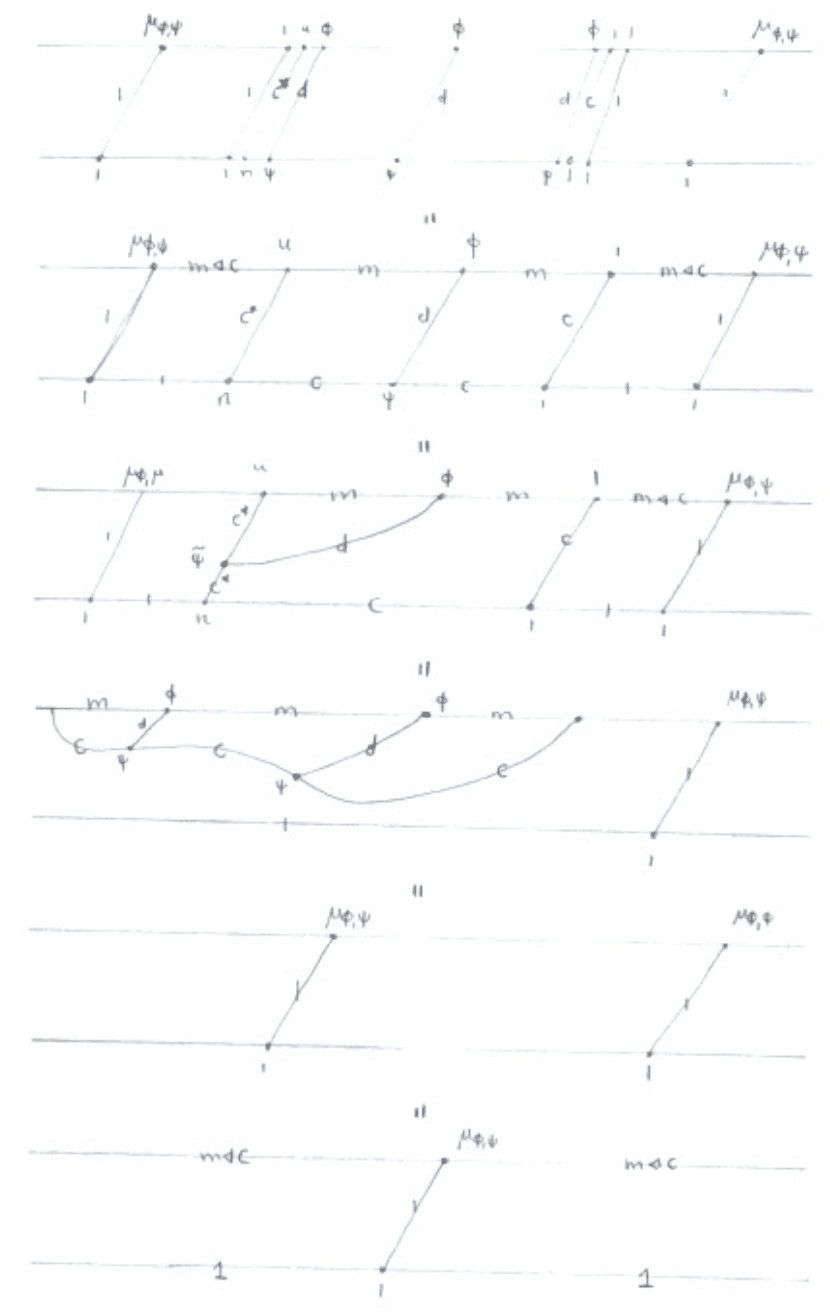
\includegraphics[width=8cm]{4}
    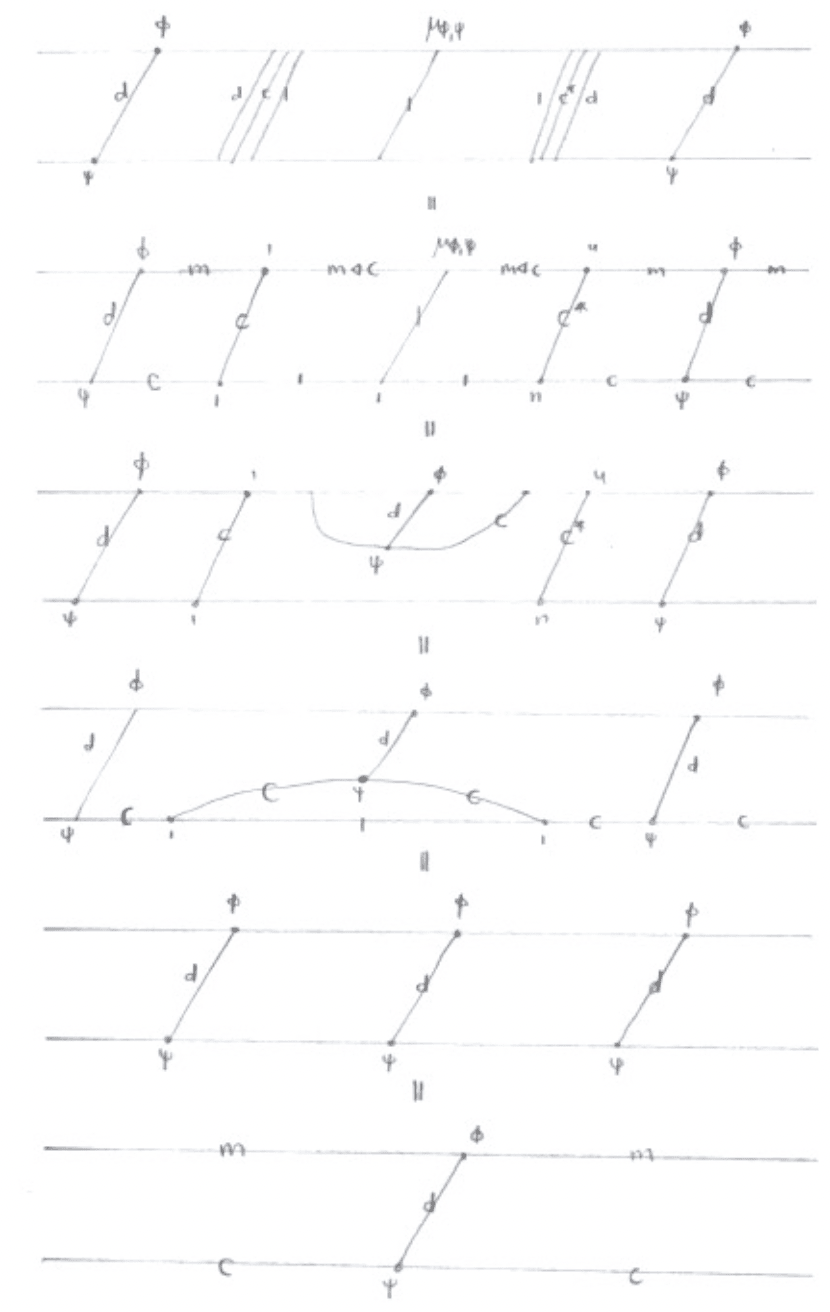
\includegraphics[width=8cm]{5}
  \end{center}
\end{proof}

\noindent For computation purpose (cf. sec \ref{section/applications}), one
may find the following basis theorem useful.

% TODO I think this is the only place we need semisimplicity and finiteness?
% We many have to fix the definition of skein category as well (it's currently
% defined on simple ones and extend by direct sums), if we are to remove the
% assumptions. // EDIT: Actually no, ss and finiteness makes Deligne products
% easier to handle.
\begin{proposition} (Basis Theorem) \label{proposition/basis-theorem}

  \noindent Let $C$ be a finite, semisimple tensor category, and
  $M_{C}, _{C}N$ be finite, semisimple module categories over $C$. \quad Thus
  the vector spaces $Hom_{M}(m, m' \lhd c), Hom_{N}(c \rhd n, n')$ have finite bases
  $\beta(m, m' \lhd c), \beta(c \rhd n, n')$ respectively. \quad Then the hom space
  $Hom_{p.sk(M,C,N)}(m \boxtimes n, m' \boxtimes n')$ has a linear basis
  \[
    \bigsqcup_{c \in Irr(C)} \beta(m, m' \lhd c) \times \beta(c \rhd n, n').
  \]
\end{proposition}
\begin{proof}
  This follows immediately from the reductions given in \ref{remark/hom-space-reduction}.
\end{proof}
